\chapter{Implementation}
\label{chap:implementation}

\section{Front end}
Viskell is started from the \code{Main} class which is only responsible for starting up the application. \code{Main} initializes a \code{CustomUIPane} and creates a \code{Scene} to which it is attached. The \code{CustomUIPane} is our extension of \code{TactilePane}, a \code{Pane} that supports multi-touch drag and drop action of its children. Zooming and panning is implemented in the \code{CustomUIPane} to extend the functionality that \code{TactilePane} offers. Variables and objects used throughout the entire application such as the \code{ConnectionCreationManager} and the Haskell environment are housed inside the \code{CustomUIPane}. The \code{CustomUIPane} is responsible for managing all underlying components and general gestures, one of these gestures is to spawn a \code{FunctionMenu}, which in turn provides the user with the ability to create other \code{Blocks}.

\subsection{Block structure}
As explained in the front end architecture, we the majority of the \code{Block's} structure is expressed in \gls{FXML}. The general structure of a \code{Block} consisted of a top level \code{BorderPane}, where the top and bottom parts contained new \code{Panes}. These top and bottom \code{Panes} where used to attach the \code{ConnectionAnchors} that the \code{Block} needed. We chose to use a naked \code{Pane} instead of a specialized \code{Pane}, this because we did not really needed the extra features a specialized \code{Pane} would offer and this provided us with direct and only control over the \code{ConnectionAnchor's} positions. This direct control was better manageable with the blocks that changed a lot in size and provided extra extensibility.

Inside the center of the top level \code{BorderPane} is the \code{Block's} content. For \code{Input-} and \code{OutputBlocks} this often results in a single element (for example a Label) representing either its input or output. \code{FunctionBlocks} makes use of a custom \code{Pane}, the \code{ArgumentSpace}, to represent its inner parts. This \code{ArgumentSpace} in turn contains several \code{InputArguments}, 1 knot and 1 output label. The \code{InputArguments} represents a single input, containing a \code{Label} and \code{InputAnchor} for that input. The knot is used to control the knot index of the function (how many inputs are applied). Finally the output label contains the current output type, the \code{OutputAnchor} is always positioned in the output space (bottom part of the top level \code{BorderPane}). These elements where positioned from left to right, where moving the knot resulted in the \code{InputArguments} fading. Features like the fading, and adjustable snapping range, were made possible by having full control from using only the bare bone \code{Pane}.

Since the information in the \code{Labels} updates often (with new type information), their length changes often as well. This results in the \code{Blocks} having to resize often. To easily make sure that everything adjusts correctly, extensive use is made of properties, a typical JavaFX addition. These properties allowed to let a single change somewhere in the \code{Block} (like a label's size) propagate to everything that was dependent on that. This also had the benefit of easier instantiation order, since everything would update till the last element was created. The extensive usage of properties resulted in a lot of positional aspects being defined in Java instead of FXML.

\subsection{Anchors}
\code{ConnectionAnchors} are used to represent input and output points of a \code{Block}. Both \code{Input-} and \code{OutputAnchors} extend \code{ConnectionAnchor}, which is implemented in such a way that both \code{Input-} and \code{OutputAnchors} need only to override a couple of methods. \code{ConnectionAnchor} keeps a list of \code{Connections} connected with him, and makes use of a primary connection concept in order to better facilitate the \code{InputAnchor}. A \code{ConnectionAnchor} has convenience methods to get an expression or string representation of its type, but these methods delegate this request to a \code{Block}. \code{ConnectionAnchors} keep track of an error state using a \code{BooleanProperty}, to which other (parts of) components can listen and react when necessary. To facilitate fat finger support, an extra invisible rectangle is attached below the visible anchor which also listens for input events for that \code{ConnectionAnchor}.

\code{ConnectionAnchors} are given an \code{AnchorHandler} to allow for user interaction with the anchors which in turn can be used to create lines. For both \code{Input-} and \code{OutputAnchors} the same \code{AnchorHandler} can be used due to the way \code{ConnectionAnchor} is structured, this mostly boils down to the function \code{canAddConnection()} that differentiates between \code{Input-} and \code{OutputAnchors}. Since multi-touch inputs only generate 3 types of events: pressed, moved and released, the same 3 events are used for \code{MouseEvents}. Although this results in not being able to use some advanced \code{MouseEvents}, this also assures us that touch can do the same as mouse, and thus allows easier testing. \code{AnchorHandler} first catches the event and extracts the necessary information for touch and mouse in separate sections, but called the same method for mouse and touch to actually do something with the event.

\subsection{Connections}
\code{Connections} are used to connect 2 \code{ConnectionAnchors}, 1 \code{Input-} and 1 \code{OutputAnchor}. \code{Connections} are visually represented using a custom extension of \code{CubicCurve}, that automatically sets the bezier points, resulting in a pretty curve instead of a straight line. A \code{Connection} also keeps track of its error state using a \code{BooleanProperty}, similar to \code{ConnectionAnchor}. Errors are visualized by adding an 'error' style class, and thus applying different CSS code to the \code{Connection}. When adding or removing anchors from \code{Connection}, changes to connectivity trigger an invalidation. \code{Connection} has lots of similar methods, to be convenient in use for both \code{Input-} and \code{OutputAnchors}.

Since supporting multi-touch means that a (or multiple) user can perform multiple actions concurrently, a \code{ConnectCreationManager} is used to link inputs to actions. \code{TouchEvents} already have an identifier, but since mouse events do not have this, a fixed identification number is assigned to \code{MouseEvents}. Using this identification number, inputs are mapped to an action that is in progress. \code{ConnectionCreationManager} then provides several methods that perform parts of what can be considered a full action. An example of an action's part would be to instantiate a new \code{Connection} with a single \code{ConnectionAnchor}, creating a \code{Connection} from an \code{InputAnchor} to an \code{OutputAnchor} is considered a full action. We chose a separate class to keep track of this in order to not have to put it in the \code{CustomUIPane} as we expected to need more similar classes in the future. Although we did not need that, it still provided useful in keeping the \code{CustomUIPane} free from clutter.

\subsection{Invalidation}
The end goal of the UI is to visually represent and interact with the back end. For that goal, the expression that is created by linking \code{Blocks} using Connections, needs to be send to the back end to evaluate it and get the result. In order to correctly and efficiently push calls to the back end and process the result of it, an invalidation scheme is implemented using several phases. In these phases an integer is used to represent the state a \code{Block} is in, namely connection state and visual state. This state can then be used to prevent duplication when traversing the tree of \code{Blocks} and even possible cycles.

The first phase of invalidation is entered upon a change in connection state, caused by either connecting or disconnected a \code{Connection} somewhere in the program (Figure \ref{fig:invalidation}:0). This will change the connection state property of the \code{Blocks} involved and in turn trigger a cascading reaction (Figure \ref{fig:invalidation}:1). A \code{Block} first has a chance to react on the state change, and then tells all the \code{Blocks} that are dependent on him (use his output) of the change, by setting their connection state to the new value. When the state change can no longer be cascaded further, the next phase is entered.

After the connection state change reaches its end, the entire expression tree gets analysed. If everything goes well, this results in types being inferred for all the expressions in each \code{Block}. When it does not go well, if a type mismatch occurs, the faulty input gets localized using the exception thrown and a mapping of expressions to \code{FunctionBlocks} (Figure \ref{fig:invalidation}:2). The input responsible for the error gets an error state, and execution of the program is halted. Since this way only 1 error can be detected at a time, previous errors are remembered whenever possible to give as much information as possible. When the expression is analysed, either correctly or incorrectly, the next phase is entered.

After having found the end of the expression and having inferred (insofar possible) its types, it is time to update the visual representation. Similar to the way the connection state cascaded, a visual state is propagated in reverse direction (Figure \ref{fig:invalidation}:2). Each \code{Block} then also reacts whenever this visual update happens, updating its labels. When the visual state can propagate no further, the invalidation is done.

Using this system it is assured that all the \code{Blocks} are fully updated before updating their visually representation and expressions are only updated and analysed when needed, separate trees won't trigger recalculation for each other.

\begin{figure}[h]
	\centering
	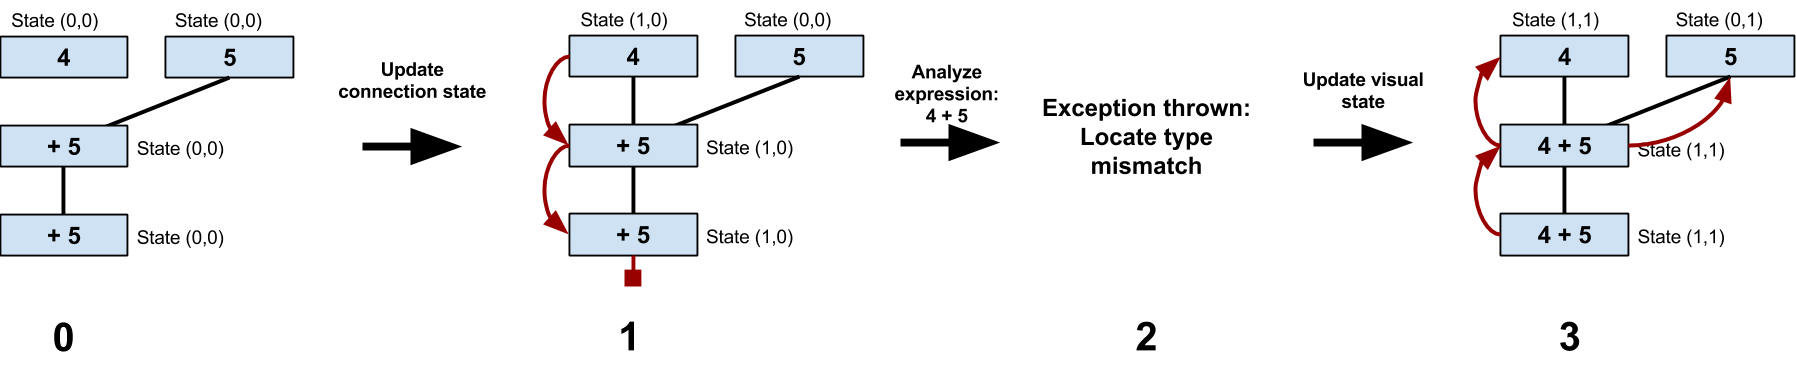
\includegraphics[scale=0.23]{Images/invalidation}
	\label{fig:invalidation}
	\caption{Invalidation scheme}
\end{figure}

\subsection{Menus}


\section{Back end}

\subsection{GHC integration}

The front end enables the user to construct Haskell expressions in a convenient manner.
The visual representation is converted into a tree of expression (\code{Expr}) objects and passed to the back end. \index{Expr}
The back end, finally, integrates with the Glasgow Haskell Compiler (\gls{GHC}) to do the actual computation.

The GHC integration is very simplistic.
The back end launches an instance of GHCi, the interactive read-eval-print-loop. \index{REPL}
This \gls{REPL} is then drip-fed the expressions over its standard input stream, converted from the intermediate representation into actual Haskell program code.
If the expression compiles and executes without problems, the result is returned to the front end.

\subsection{Expression and type representation}

\begin{figure}[h]
	\centering
	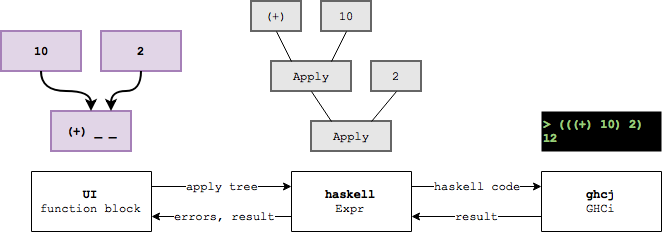
\includegraphics[scale=0.5]{Images/exprtohaskell}
	\label{fig:classdiagram-expr}
	\caption{Translation from visual representation to Haskell code}
\end{figure}

\subsubsection{Expressions}
\index{function} \index{Haskell code}

To be able to work with Haskell code in Java, we built our own representation for the Haskell programming language.
We have chosen to use distinct classes (with a common superclass) for expressions that behave in a similar manner.
This object-based approach is favoured over any text based approach (including using Haskell code itself) because objects are very easy to work with.

Every expression is represented as an instance of \code{Expr} (or any subclass of \code{Expr}). \index{Expr}
An \code{Expr} is responsible for outputting syntactically correct Haskell code. \code{Expr} objects are the bridge between the tree-like graphical representation of the user interface and the textual Haskell code.
The implemented types of expressions are standard functions, values and function applications.
Each of these types of expressions share the fact that they all have a type which can be used by the type checker.

Standard functions (functions that are known to the Haskell environment) are represented as an \code{Ident} instance. \index{Ident}
This class is very simple and does not include more than the name of the function (so it can be called) and a way to lookup the type.

Values are represented in a similar way, a \code{Value} object keeps track of the string representation of the value and its type. \index{Value}
The string representation of the value should be written in a way that GHCi natively understands what is meant by it, altough this is not validated.

Function application is done by using an \code{Apply} object. \index{Apply}
This class holds two expressions where the second expression is applied to the first expression.
\code{Apply} is limited to the application for a single argument.
A function with more than one argument is seen as a function with one argument that produces another function.
This way \code{Apply} allows for creating a tree like structure of a Haskell program.

Custom functions can be built using a composition of standard functions.
A custom function is defined using a \code{Function} object.
This object requires a specification of the function arguments and the expression tree of the function.
A \code{FunctionArgument} object can be used in this expression tree to use the inputs.
Functions that are defined this way will make sure that type calculations are done on a per-usage basis so reusing a function is always possible.
When a function is pushed to GHCi an \code{Ident} object is given which can be used instead of the \code{Function} object.
This comes with a great performance gain because the function itself is not continuously type checked.

Once a program has been represented as a tree of \code{Expr} objects, calling the \code{Expr.analyze()} method will invoke the type checker.
The type checker calculates the new types for the expressions in the tree.
The new types of each expression can be obtained by calling the \code{Expr.getType()} method.
This way it is possible to always get the up-to-date type of an \code{Expr} object by simply keeping a reference to it.

\begin{figure}[h]
\centering
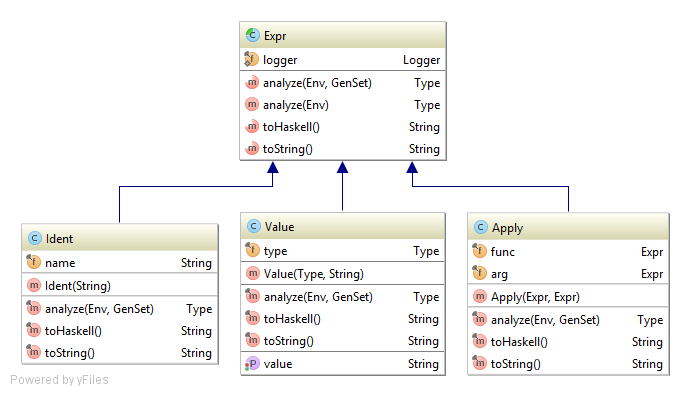
\includegraphics[scale=0.4]{Images/classdiagram-expr}
\label{fig:classdiagram-expr}
\caption{Class diagram of the Haskell expressions classes}
\end{figure}

\subsubsection{Types}
\index{type}

Types are represented similarly to expressions.
Each type is represented as an instance of \code{Type} (or any subclass of it).
The subclasses of \code{Type} are used to make working with types easier.
There is no subclass for every distinct type in Haskell, only for groups of types that are alike.

First of all types are separated into two groups: variable types and nonvariable types.
Variable types are types of which the actual type is not known - types that can unify into any nonvariable type (possibly with constraints).
Variable types are represented as \code{VarT}.

Nonvariable types (constant types) are represented as \code{ConstT} and consist of a type constructor and a number of (optional) argument types.
A type is considered constant when it is clear which type constructor to use. A type with a known type constructor but variable types as argument types is still a constant type.

Composite types, e.g. list and tuple, are represented by respectively \code{ListT} and \code{TupleT} which are subclasses of \code{ConstT}.
These subclasses handle some validation and Haskell/string representation that is specific to these types.

Distinct Haskell types are represented as class instances, not as the class itself. The different \code{Type} subclasses make it easier to work with the types, and some are necessary in case of compound types like \code{ListT} and \code{TupleT} which are special cases.

Non-variable types can be easily compared. Two instances of the same type are equal (that is, two instances with the same base class and constructor arguments).
Variable types are only equal if it is the same instance. This is used to avoid confusion between variable types with the same name.

Type classes are represented as \code{TypeClass} instances and can be used as constraints on variable types.
Each \code{TypeClass} instance keeps a set of constant types that belong to the type class.
This information is used by the type checker to check whether a variable type is unifyable with a constant type or another variable type.

\begin{figure}[h]
\centering
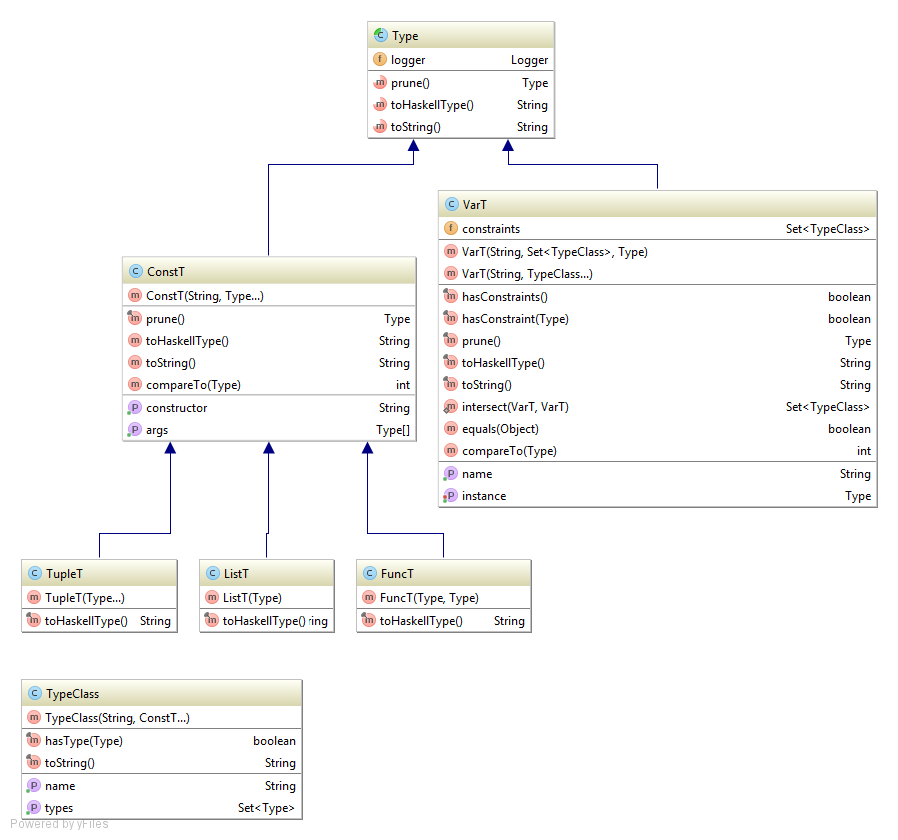
\includegraphics[scale=0.4]{Images/classdiagram-type}
\label{fig:classdiagram-type}
\caption{Class diagram of the Haskell types classes}
\end{figure}

\subsection{Type checker}
\index{type checker}

From our own experience as beginning Haskell programmers, we often encountered type errors, and therefore GHC's type error messages.
Very early in the project, we decided that the back end had to do at least some type-related work itself, to provide better errors to the user, and also to be able to show type hints, without having to parse GHC's error messages.
Not long thereafter, it was decided that such a home-grown type checker would not need to support the entirety of Haskell's type system.

After some iterations, we have arrived at an approach that could probably be described as a subset of Hindley-Milner type inference. \index{Hindley-Milner} \index{type inference}

Our (Java) implementation of Hindley-Milner type inference is based on an implementation in Scala by Andrew Forrest\cite{forrest}.
This implementation was in turn based on an implementation in Perl by Nikita Borisov\cite{borisov}.
The Perl implementation was heavily inspired by a Modula-2 implementation from 1987 by Luca Cardelli\cite{cardelli}.
Some ideas were also taken from the chapter on types from the programming languages book by Krishnamurthi\cite{plai}.

As mentioned, the type checker is not nearly powerful enough to understand or even represent the entire complexity of Haskell's type system.
However, we have found it to be `good enough' for our purposes.

\subsection{Environment management}
\index{catalog}
\index{environment}

In Haskell a lot of things depend on the environment, for example the functions that are available, the types in type classes, etc.
Our implementation solves this by introducing an environmet (\code{Env}).
Objects of this class keep the types of the available functions and the type classes for every type.
Furthermore, we provide a XML-based catalog where the initial functions and type classes can be configured.
This catalog contains information that can be used by the front end, such as documentation as well.
